\section{Existing solutions}
This section will discuss some of the existing solutions used for video surveillance, such as regular camera, photo sensor, and dome camera.
The strengths and weaknesses of each solution will be covered.
The figures referenced in this section show the same area with a different surveillance setup to make them comparable. \\

In a regular camera solution mounted cameras are used.
These cameras surveil a limited area, and in order to cover a larger area, multiple cameras are needed.
Multiple areas can be surveilled simultaneously with multiple cameras.
A limitation with a regular camera setup is that the cameras are stationary.
This means a cameras field of view can be limited by physical objects.
In Figure~\ref{} it can be seen how an object is placed in a camera's field of view, which creates a blind spot in an area that the camera would normally cover.
As an example in Figure~\ref{fig:refular_camera_setup} it can be seen how an object placed in a cameras field of view can create a blind spot in an area normally covered by a camera. \\

\begin{figure}[htb]
    \centering
    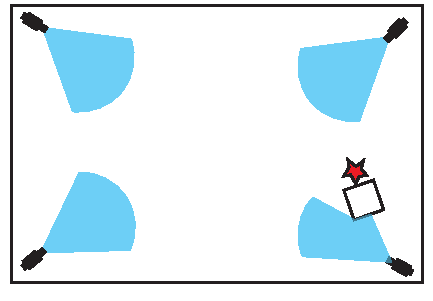
\includegraphics[width=0.7\textwidth]{gfx/regular_camera_setup.pdf}
    \caption{Example of a Regular Camera Setup.}
    \label{fig:refular_camera_setup}
\end{figure}

%\fixme{Figuren i billedet skal rykkes mere ind i kameraets view.}

The red star in Figure ~\ref{fig:refular_camera_setup} represents a critical object, that needs to be observed. \\

In a photo sensor solution the perimeter of the surveilled area is covered by both cameras and photo sensors.
The purpose of the setup is to detect if anything enters the area, and then activate the cameras to capture it on video as seen in Figure~\ref{fig:photo_sensor}.
A photo sensor solution can be used in combination with a regular camera solution, to surveil both the interior and the perimeter of an area.
The advantage of a photo sensor setup is that the cameras surveilling the perimeter are only activated if the sensors are triggered, ensuring video footage is only recorded when it is needed.
The disadvantage is that the cameras are still stationary, meaning a large amount of cameras are required to surveil a large area. \\

\begin{figure}[htb]
    \centering
    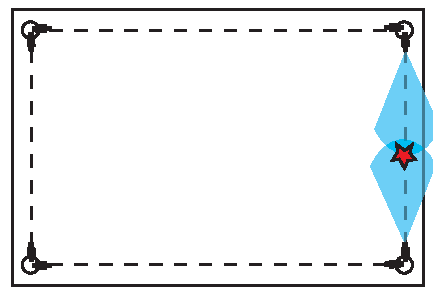
\includegraphics[width=0.7\textwidth]{gfx/light_sensor.pdf}
    \caption{Example of a Photo Sensor Setup.}
    \label{fig:photo_sensor}
\end{figure}

The next solution has a dome camera with a long field of view positioned in the center.
The perimeter is then divided into zones, by e.g. photo sensors.
When a zone has detected an entry, the dome camera is rotated towards that zone to observe the area.
Compared to the two previous solutions, the dome camera solution is limited to observing a specific subarea at a time as seen in Figure~\ref{fig:drone_sensor}. \\

\begin{figure}[htb]
    \centering
    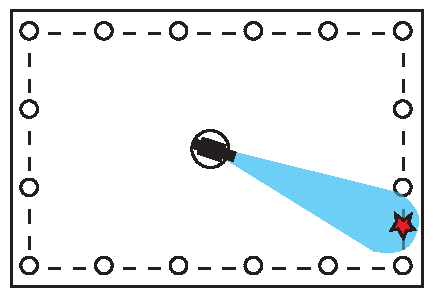
\includegraphics[width=0.7\textwidth]{gfx/drome_sensor.pdf}
    \caption{Example of a Dome Setup.}
    \label{fig:drone_sensor}
\end{figure}
